\section{Verlet Integrator}
The goal of this part is to derive a first simple algorithm to integrate the equations of motion.

\subsection{Hamilton equations}
    \subsubsection{Hamilton equations for one particle in $1D$}
        Let's consider a system made of one particle moving in a one-dimensional space. Let $q$ be its coordinate and $p$ its momentum. The Hamiltonian $H(p,q)$ of this system satisfies the following equations, that we usually call the \textit{\textbf{Hamilton equations}}:
        \begin{equation}
        \begin{cases}
            \dot{q}=\frac{\partial H}{\partial p}\\
            \dot{p}=-\frac{\partial H}{\partial q}
        \end{cases} \label{hamiltoneq}
        \end{equation}
        For the vast majority of the systems we would be interested in, we can write:
        \begin{equation}
            H=K(p)+U(q)
        \end{equation}
        where $K$ is the kinetic energy of our system and $U$ is its potential energy.
        \\ Then the Hamilton equations \eqref{hamiltoneq} become:
        \begin{equation}
        \begin{cases}
            \dot{q}=\frac{\partial K}{\partial p}\\
            \dot{p}=-\frac{\partial U}{\partial q}
        \end{cases}
        \end{equation}
        In the cases we will be mostly interested in, we can also write the kinetic energy as:
        \begin{equation}
            K=\frac{p^2}{2m}
        \end{equation}
        where $m$ is the mass of the particle.
        \\ Hence:
        \begin{equation}
            \dot{q}=\frac{\partial H}{\partial p}=\frac{\partial K}{\partial p}=\frac{p}{m}
        \end{equation}
        Moreover, we usually have:
        \begin{equation}
            \dot{p}=-\frac{\partial U}{\partial q}=f
        \end{equation}
        where $f$ is the force acting on our particle.
        \\ Whence the usual form of the Hamilton equations for one particle in $1D$ is actually:
        \begin{equation}
        \begin{cases}
            \dot{q}=\frac{p}{m}\\
            \dot{p}=f
        \end{cases}
        \end{equation}
        
    \subsubsection{Hamilton equations for $N$-particles systems in $3D$}
        All the equations we have written for a single-particle system can be generalized to a system made of $N$ particles. To do so, we just have to add a subscript $i \in  [\![ 1;N ]\!]$ to the quantities $q$, $p$, $m$ and $f$, that depend on each of the particle.
        \\Hence, for a system with $N$ particles moving in one dimension, we have $2N$ Hamilton equations, corresponding to the positions $q_i$ and the momenta $p_i$ of each of the particles that form the system:
        \begin{equation}
        \begin{cases}
            \dot{q_1}=\frac{\partial H}{\partial p_1}=\frac{\partial K}{\partial p_1}=\frac{p_1}{m_1}\\
            \dot{p_1}=-\frac{\partial H}{\partial q_1}=-\frac{\partial U}{\partial q_1}=f_1\\
            \hfil \vdots\\
            \dot{q_N}=\frac{\partial H}{\partial p_N}=\frac{\partial K}{\partial p_N}=\frac{p_N}{m_N}\\
            \dot{p_N}=-\frac{\partial H}{\partial q_N}=-\frac{\partial U}{\partial q_N}=f_N
        \end{cases}
        \end{equation}
        Notice that now, the kinetic energy $K$ of the system is:
        \begin{equation}
            K=\sum_{i=1}^N\frac{p_i^2}{2 m_i}
        \end{equation}
        If our particles are moving in a three-dimensional space, we have to add another index $j \in  \{ x,y,z \}$ (or $j \in  \{r,\theta,\phi\}$, depending on the coordinate system used), that indicates the space coordinates of the positions and the momenta of each of the particles. Hence we have $6$ equations describing each particle $i$; for instance, in the Cartesian coordinate system:
        \begin{equation}
        \begin{cases}
            \dot{q}_1^{x,y,z}=\frac{\partial H}{\partial p_1^{x,y,z}}=\frac{\partial K}{\partial p_1^{x,y,z}}=\frac{p_1^{x,y,z}}{m_1}\\
            \dot{p}_1^{x,y,z}=-\frac{\partial H}{\partial q_1^{x,y,z}}=-\frac{\partial U}{\partial q_1^{x,y,z}}=f_1^{x,y,z}
        \end{cases}
        \end{equation}
        We have therefore in total a system of $6N$ equations describing an $N$-particles system in a three-dimensional space. We can lighten the script by writing $\textbf{q}=(q_x,q_y,q_z)$, $\textbf{p}=(p_x,p_y,p_z)$ and $\textbf{f}=(f_x,f_y,f_z)$, and then simply considering vector equations. That's why we won't consider the space-dimensional index in what follows.
        
        \subsubsection{Connection between Newton's second law of motion and Hamilton equations}
        Let's consider the Hamilton equations describing a given particle $i$:
        \begin{equation}
            \begin{cases}
                \dot{q_i}=\frac{p_i}{m_i}\\
                \dot{p_i}=f_i
            \end{cases}
        \end{equation}
        Then:
        \begin{equation}
            \ddot{q_i}=\frac{d}{d t}(\frac{p_i}{m_i})=\frac{\dot{p_i}}{m_i}
        \end{equation}
        since $m_i$ is assumed to be independent of time.
        In other words:
        \begin{equation}
            \ddot{q_i}=\frac{f_i}{m_i}
        \end{equation}
        which is nothing but the Newton's second law of motion!
        \\Hamilton equations and Newton's second law are two different but totally equivalent formulations.
        \begin{itemize}
            \item Hamilton equations are first order differential equations where we have two variables for every particle and every dimension: for a system of $N$ particles in $3D$, we have $6N$ first order differential equations.
            \item Newton's equations are second order differential equations with a single variable for each particle and each dimension: for a system of $N$ particles in $3D$, we have $3N$ second order differential equations.
        \end{itemize}
        In most of the cases, it will be more convenient for us to use the Hamilton equations. The reason is practical: it's easier to derive a finite time step integrator for first order equations.
    
    \subsubsection{Phase space}
    The phase space is the space $(q,p)$ of all possible values of positions and momenta of the system. We can draw the phase space only for a single particle moving in a one-dimensional space, since the dimension of the phase space is equal to $2 \times N \times D$, where $N$ is the number of particles, $D$ is the dimension of the space and $2$ comes from the fact that for each particle and each dimension, we have to represent the position $q$ and the momentum $q$, \textit{i.e.} $2$ variables.
    \\$(q(t),p(t))$ is the trajectory of the system in the phase space.
    \\ Let's see what happens to the dynamics of a particle in the phase space for a very special and simple case: the harmonic oscillator (HO) in 1D.
    \\ For a HO 1D, we have:
    \begin{equation}
        \begin{cases}
            K_{HO}=\frac{p^2}{2m}\\
            U_{HO}=\frac{k q^2}{2}
        \end{cases}
    \end{equation}
    Then the Hamilton equations are:
    \begin{equation}
        \begin{cases}
            \dot{p}=-kq\\
            \dot{q}=\frac{p}{m}
        \end{cases}
    \end{equation}
    By solving the Hamilton differential equations, we obtain the trajectory of the system in the phase space, which is an ellipse. If we set $m=1$ and $k=1$, the trajectory is a circle.
    
    \subsubsection{TIME REVERSIBILITY}
    The time-reversed (or backward) trajectory of the system is $(q(-t),-p(-t))$. Let's show that the Hamilton equations are time-reversible, \textit{i.e.} if the forward trajectory is a solution of the Hamilton equations, then the backward trajectory is also a solution of the same Hamilton equations.
    \\Let $q^*(t)=q(-t)$ and $p^*(t)=-p(-t)$.
    \begin{equation}
        \frac{d}{dt}q^*(t)=\frac{d}{dt}q(-t)=-\frac{d}{d(-t)}q(-t)=-\frac{\partial H}{\partial p}(-t)=\frac{\partial H}{\partial (-p)}(-t)=\frac{\partial H}{\partial p^*}(t)
    \end{equation}
    We can do the same for $p^*$. Consequently, to sum up:
    \begin{equation}
        \begin{cases}
            \frac{d}{dt}q^*(t)=\frac{\partial H}{\partial p^*}(t)\\
            \frac{d}{dt}p^*(t)=-\frac{\partial H}{\partial q^*}(t)
        \end{cases}
    \end{equation}
    Then $(p^*,q^*)$ is also a solution of the Hamilton equations and the equations are time-reversible.
    \\What is the physical interpretation of time reversibility? Let's take again the example of the HO.
    These two trajectories are not identical: one is the time-reversed of the other. As Hamilton equations are reversible, both trajectories are actually solutions of the same Hamilton equations but with different initial conditions. Time-reversibility implies that we can't distinguish between a given trajectory and its time-reversed one: if we take a trajectory, then time-reverse it and give the time-reversed trajectory to someone else, they won't be able to say whether it has been time-reversed or not just by observing it.
    
    \subsubsection{ENERGY CONSERVATION}
    Let's assume that the Hamiltonian doesn't depend explicitly on time but only on $q$ and $p$, \textit{i.e.} $H=H(q,p)$. For instance, in the case of the HO, we assume that $m$ and $k$ don't change in time.
    \\For a single particle, we have:
    \begin{equation}
        \frac{dH}{dt}=\frac{\partial H}{\partial q} \frac{\partial q}{\partial t} + \frac{\partial H}{\partial p} \frac{\partial p}{\partial t}
    \end{equation}
    More generally, with $N$ particles:
    \begin{equation}
    \begin{aligned}
        \frac{dH}{dt}&=\sum_{i=1}^N \left( \frac{\partial H}{\partial q_i} \frac{\partial q_i}{\partial t} + \frac{\partial H}{\partial p_i} \frac{\partial p_i}{\partial t} \right)\\&=\sum_{i=1}^N \left( \frac{\partial H}{\partial q_i} \dot{q_i} + \frac{\partial H}{\partial p_i} \dot{p_i} \right)\\&=\sum_{i=1}^N \left( \frac{\partial H}{\partial q_i} \frac{\partial H}{\partial p_i} - \frac{\partial H}{\partial p_i} \frac{\partial H}{\partial q_i} \right)\\&=0
        \end{aligned}
    \end{equation}
    where the third equality is obtained thanks to the Hamilton equations. Hence $H$ is a function of the point in the phase space but its value doesn't change when we follow a trajectory.
    \\Then, for a HO, we have:
    \begin{equation}
        H=\frac{p^2}{2m}+\frac{kq^2}{2}=const
    \end{equation}
    \textit{I.e.}, with $m=1$ and $k=1$:
    \begin{equation}
        p^2+q^2=const
    \end{equation}
    As $\sqrt{p^2+q^2}$ is the distance of the point $(q,p)$ to the origin of the graph,we move along a circle when following a trajectory.
    \\Energy conservation is a general property of the Hamilton equations, which is not specific to harmonic oscillators. If we have a $1D$-system with a potential which is not a quadratic function, the trajectory will still be a Hamiltonian isoline, but with a different shape.
    \\In higher dimension, the trajectory is also a line but, if we put together all the points of the phase space that have the same value of $H$, we won't have a line anymore, but a hypersurface. As the phase space has in general $6N$ dimensions ($N$: number of particles), the union of all the points that have the same value of energy is a $(6N-1)$-dimensional space (we have one constraint, which is the equation $H(q_i,p_i)=const$). The trajectory is a line on that hypersurface. For instance, for a multi-dimensional HO, the hypersurface is a sphere and the trajectory is a line on this sphere.
    
\subsection{Verlet Algorithm}
    How to solve the equations of motion numerically?
    \\Let's start with Newton's second law:
    \begin{equation}
        \ddot{q}=\frac{f}{m}\label{newton_second}
    \end{equation}
    Now, let's do a Taylor expansion of $q$ as a function of $t$:
    \begin{align}
        q(t + \Delta t) \underset{\Delta t \to 0}{=}q(t)+\dot{q}(t)\Delta t+\frac{\ddot{q}(t)}{2}\Delta t^2+\frac{\dddot{q}(t)}{6}\Delta t^3+O(\Delta t^4) \label{tayexp_q_plus}\\
        q(t - \Delta t) \underset{\Delta t \to 0}{=}q(t)-\dot{q}(t)\Delta t+\frac{\ddot{q}(t)}{2}\Delta t^2-\frac{\dddot{q}(t)}{6}\Delta t^3+O(\Delta t^4) \label{tayexp_q_min}
    \end{align}
    Then, let's sum \eqref{tayexp_q_plus} and \eqref{tayexp_q_min}. As the odd-derivatives terms cancel each other (notice that $\dot{q}(t)=v(t)$ disappears), we obtain:
    \begin{equation}
        q(t + \Delta t)+q(t - \Delta t)\underset{\Delta t \to 0}{=}2q(t)+\ddot{q}(t)\Delta t^2+O(\Delta t^4) \label{just_bef_verlet}
    \end{equation}
    Given \eqref{newton_second}, we can finally write the expression of what we call the \textbf{VERLET ALGORITHM}:
    \begin{equation}
        \boxed{q(t+\Delta t)\underset{\Delta t \ll 1}{\simeq} 2q(t)-q(t-\Delta t)+\frac{f(t)}{m}\Delta t^2}\label{verlet_algo}
    \end{equation}
    This algorithm is one of the simplest and most common way to integrate the Hamilton or Newton equations of motion.\\
    To compute $q(t+\Delta t)$, we need to compute the force $f$ acting on the particle.
    \begin{equation}
        f(t)=-\frac{\partial U}{\partial q}
    \end{equation}
    Let's assume that $U$ doesn't depend explicitly on time. Then $U=U(q(t))$ and compute the force using only the current value of the position $q(t)$ (and not, for instance, the previous values or something else).\\
    For instance, let's take a free particle. Here, $f=0$  and the Verlet expression \eqref{verlet_algo} is then:
    \begin{equation}
        q(t+\Delta t)=2q(t)-q(t-\Delta t)
    \end{equation}
    Thus, to compute the new position $q(t+\Delta t)$, we just have to take the current position $q(t)$ and to add to it the vector\footnote{Here, \textit{vector} is used in a large mathematical sense: in $1D$, it's just a number.} $[\mathbf{q}(t)-\mathbf{q}(t-\Delta t)]$, as shown in the Figure \ref{fig:verlet_freepart}.
    \begin{figure}[H]
        \centering
        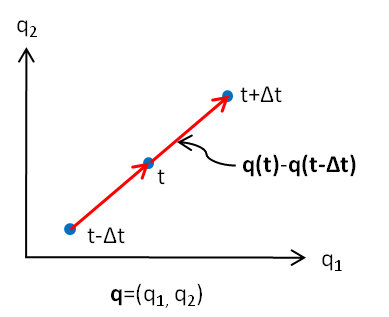
\includegraphics[width=0.6\textwidth]{Integrators/images/verlet_freepart.png}
        \caption{Position $q(t+\Delta t$) of a free particle in $2D$ computed using Verlet algorithm}
        \label{fig:verlet_freepart}
    \end{figure}
    \noindent We can notice that computing the new position amounts to nothing but extrapolating the trajectory. Of course, if $f\neq 0$, the system behaves differently; however, we can say as a first approximation that the system actually just extrapolates, but with a correction due to the force acting on it.
    \\Now, we can code the Verlet algorithm:
    \begin{algorithm}[H]
		\caption{Verlet Algorithm}
        \label{alg:verlet}
		\begin{algorithmic}[1]
		    \State $qo,q=...~~\#initialization$ 
		    \For{$i=1,...,nsteps$}
			\State $qn=2q-qo+f(q)*dt^2/mass$ 
			\State $qo=q$
			\State $q=qn$
			\EndFor
			\State $\# dt: time step\leftrightarrow \Delta t~;~qo: old position\leftrightarrow q(t-\Delta t)~;~qn: new position\leftrightarrow q(t+\Delta t)~;~q: current position\leftrightarrow q(t)$
		\end{algorithmic}
	\end{algorithm}
	\noindent In this algorithm, we don't start with initial position and velocity, but with the initial position $q=q(t_0)$ and the position just before $qo=q(t_0-\Delta t)$. Actually, $q-qo$ contains in some way the information about the velocity, but it's not trivial. Anyway, the amount of information is well and truly the same. In fact, there's no velocity in this algorithm; we will see another one where velocity appears in the next section~(\ref{sec:velocity_verlet}).
	\\An algorithm is discrete in time and, of course, the trajectories we obtain using Verlet algorithm are actually not exact solutions of the Hamilton equations. Then we can wonder whether these trajectories satisfy even so the properties of Hamilton equations. Let's check.
	
    \subsubsection{Time reversibility}
    \textbf{The solutions obtained using Verlet algorithm are time-reversible.} Indeed, as $q(t+\Delta t)$ and $q(t-\Delta t)$ play perfectly symmetric roles in the algorithm equation\eqref{verlet_algo}, the trajectories obtained using Verlet algorithm are exaclty time-reversible, even if $\Delta t$ is not small. In other words, there's no reversibility breaking in Verlet algorithm, \textit{i.e.} there's no error in time-reversibility with Verlet algorithm.
    
    \subsubsection{Energy conservation}
    Is the energy conserved by Verlet algorithm? As in this algorithm there's no velocity, we can't compute the energy and \textbf{we can actually not answer this question here}... In the next section~(\ref{sec:velocity_verlet}), we will see an algorithm which is equivalent to the present one and where there is the velocity, so that we are able to compute the energy and to check whether it is conserved or not (spoiler: it is not!). Of course, this inability to check energy conservation is a flaw but, as we will see, it's not the biggest disadvantage of Verlet algorithm.
    
    \subsubsection{Formal errors}
    As in the Verlet algorithm expression \eqref{verlet_algo} the terms $\pm \frac{1}{6}q(t)\Delta t^3$ coming from \eqref{tayexp_q_plus} and \eqref{tayexp_q_min} cancel each other, the only mathematical errors come when we go from \eqref{just_bef_verlet} to \eqref{verlet_algo}. However, these mathematical errors that are of the order of $\Delta t^4$ and accumulate at every step are not the only ones that affect the solution we obtain: indeed, as we are using a computer, we also have to take into account numerical roundoff errors.
    
    \subsubsection{Roundoff errors}
    A computer can store a finite number of digits. For example, in single-precision, \textit{i.e.} in a 32-bits system, the biggest integer the computer can represent is $2^{32}-1=(\underbrace{111...111}_{32~digits~1})_2$. As regards floats, the number of significant digits is of course also limited. For instance, single-precision floats, have about $7$ significant digits in base $10$ and therefore, if we sum two floats, a big one and a much smaller one, whose ratio is less than $10^{-7}$, the computer neglects the small one with respect to the big one and the sum is set equal to the big number.
    \\In general, people actually ignore these roundoff errors. But if this is pretty fair when using a double-precision format, \textit{i.e.} 64-bits, since we have there about $16$ significant digits in base $10$, we would better be quite careful in single-precision.
    \\In the case of Verlet algorithm, we must actually be always careful. Indeed, as we can see in the equation \eqref{verlet_algo}, in order to compute $q(t+\Delta t)$, we have to add to $(q(t)+\frac{f(t)}{m}\Delta t^2)$ the difference $(q(t)-q(t-\Delta t))$. Yet this difference is very small and the computer would tend to set it equal to $0$: if the difference is less than $10^{-6}$ times $(q(t)+\frac{f(t)}{m}\Delta t^2)$, it will be effectively $0$ in single-precision. \textit{De facto}, the smaller is the time step $\Delta t$ we choose, the bigger are this effect and then the usually ignored numerical roundoff errors we were speaking about just before. Here we have actually a kind of paradox, since when decreasing $\Delta t$ increases numerical errors, it is in the same time the only way to decrease the formal mathematical errors.
    \newline
    \\To put it in a nutshell, even it is very simple and quite popular, the Verlet algorithm we derived in this section is actually not that well, as it is very sensitive to roundoff numerical errors.
    
\subsection{Liouville formalism}

    Now, instead of describing the evolution of a single copy of our system, let's describe the evolution of many copies of the system. We have thus to repeat the calculations for many initial conditions and describe the properties of a set of trajectories. To do so, we can partition the phase space into small cubes and count how many copies of the system are in each small cube thanks to a density function $\rho(X,t)$, which is the number of copies of the system belonging to the square with coordinates $X$. $X=(p_i,q_i)$ is a vector in $6N$ dimensions, where $N$ is the number of atoms forming the system. Whence $\rho$ is a very complicated object.
    \\To begin, we initialize many copies of the system in different places - or even all in the same place: that corresponds to the initial value of $\rho$, which counts the number of copies of the system in each point of the phase space. Then we propagate each of the copies using Hamilton equations and see how $\rho$ is changing in time; in other words, we see each copy of the system moves through Hamilton equations.
    \\Let's set $\dot{X}_i=(\dot{p}_i,\dot{q}_i)=v_i$ the phase space velocity, which is not the physical velocity but the rate at which $p$ and $q$ change in time.
    \\We can also define a current density  $J_i(X)=\rho(X) v_i(X)$. As what we are integrating is a differential equation on $X$, there should be no jump in the trajectory of $X$ and we can assume that $X$ evolves in a continuous manner. Then the density and the current are well defined and we can compute the rate of change of $\rho$:
    \begin{equation}
    \begin{aligned}
        \frac{\partial \rho (X,t)}{\partial t}&=-\nabla \cdot \mathbf{J}=-\sum_i\frac{\partial}{\partial X_i}J_i=-\sum_i\frac{\partial}{\partial X_i}(\rho v_i)=\\
        &=-\sum_i\frac{\partial}{\partial q_i}(\rho \dot{q}_i)-\sum_i\frac{\partial}{\partial p_i}(\rho \dot{p}_i)=\\
        &=-\sum_i\frac{\partial \rho}{\partial q_i}\dot{q}_i-\sum_i\frac{\partial \rho}{\partial p_i}\dot{p}_i-\sum_i\frac{\partial \dot{q}_i}{\partial q_i}\rho-\sum_i\frac{\partial \dot{p}_i}{\partial p_i}\rho\\
    \end{aligned}
    \end{equation}
    Now, according to Hamilton equations, we have:
    \begin{equation}
        \begin{cases}
            \dot{q}_i=\frac{\partial H}{\partial p_i}\\
            \dot{p}_i=-\frac{\partial H}{\partial q_i}
        \end{cases}
    \end{equation}
    Whence:
    \begin{equation}
        \frac{\partial \rho (X,t)}{\partial t}=-\sum_i\frac{\partial \rho}{\partial q_i}\dot{q}_i-\sum_i\frac{\partial \rho}{\partial p_i}\dot{p}_i-\cancel{\sum_i\rho \frac{\partial^2 H}{\partial q_i\partial p_i}}+\cancel{\sum_i\rho \frac{\partial^2 H}{\partial p_i\partial q_i}}
    \end{equation}
    Finally, we have:
    \begin{equation}
        \frac{\partial \rho (X,t)}{\partial t}+\sum_i\frac{\partial \rho}{\partial q_i}\dot{q}_i+\sum_i\frac{\partial \rho}{\partial p_i}\dot{p}_i=0
        \label{just_bef_liouville}
    \end{equation}
    The first term tells us how the density changes because $t$ is flowing and the two last terms tell us how it changes if we follow a trajectory. Indeed, even if we stay always at the same point in the phase space, the density changes because some other copies of the system are coming in and out.
    \\If we rewrite the equation \eqref{just_bef_liouville} using the total derivative of $\rho$, we obtain the \textbf{LIOUVILLE THEOREM}:
    \begin{equation}
        \boxed{\frac{d\rho}{dt}=0}\label{liouville_theorem}
    \end{equation}
    The total derivative of $\rho$ is equal to $0$, so that if we consider a set of copies of the system, it behaves like an incompressible flow. In other words, Liouville theorem states that the density remains constant when we follow the flux.
    \\In fact, Liouville equation contains exactly the same information as Hamilton equations. It's just more complicated because it's written in a very high-dimensional space. In another sense, as it's a linear equation in $\rho$, it's actually simpler. Liouville equation can be solved exactly: we will use its solutions to derive integrators for Hamilton equations.